\chapter{Design}
\subsection{Introduction}
In this chapter, the design of the prototype and its graphical decisions will be discussed and defined, with the requirements set in the analysis, which were further defined in the design requirements section (\ref{DesignRequirements}). When designing, different aspects will be taken into consideration for user experience - usability goals and principles (\ref{sec:UsabilityGoals}), mobile usability (\ref{MobileUsability}), establishing intuitivity through familiarity, as well as the technical side on which the user experience also depends - fluent implementation of the graphical user interface and non-traditional sensors, while also ensuring that the system performance is smooth. In further design iterations users would be involved in the design process (\ref{UserCenteredDesign}), as user centered design is one of the elements to designing a good user experience (\ref{fig:UserCenteredDesign}).

\subsection{Concept}
The goal of the prototype is to help in answering which control scheme may be the best solution for the most familiar and effective navigation in 3d environment. Designing a prototype that creates a familiar and effective navigation that is not traditional can go in various directions, but the concept was narrowed down to using just the sensors that could help establish the design requirements initiated earlier (\ref{DesignRequirements}), those being the multi-touch and the gyroscope.
To be able to design a prototype with all the necessary aspects, control schemes and a base test level for navigation in 3D virtual environment have to be designed with the established design requirements (\ref{DesignRequirements}).
The prototype has to implement two features to navigate in 3D virtual environment - the moving of the camera and the camera rotation. It was chosen to make extremities of the control schemes to establish familiarity in distinct ways. The familiarity concept will be put into effect as the control schemes for controlling the camera have to be linked with something that the user might be familiar with already. 

\subsection{Interface Design}
The currently existing sensors in mobiles enable the creation of unusual ways of controlling a 3d environment. With the goal in mind of achieving familiarity through the non-traditional sensors, two different approaches were established. The knowledge and familiarity to the currently existing products on the market (\ref{SOTA}), and the familiarity of movement representative to the one of movement in real life. For both approaches the current and the target knowledge (\ref{knowledgeSpace}), points for the user are expected to be separate. The design needs to be established in a way to help the users get through the knowledge gap intuitively, when they are involved in the designed task. It was chosen to make extremities of the control schemes to establish familiarity in distinct ways. It was important to keep the same movement speed settings for all the control schemes for later evaluations. That meant that in the perfect scenario, the user should be able to get from one position to another with the same amount of time spent for that task on each of the control schemes.

\subsection{Control Schemes}
Three distinct control schemes were designed for the navigation. Buttons-only, Joysticks-only, and one that includes buttons for moving back and forth, with a gyroscope for moving the camera. The fact that newer smart devices are capable of multi-touch input has been used as an advantage to enable both the movement and the rotation to be controlled simultaneously. That creates the possibility for the user to walk and turn around at the same time.

\subsubsection{Gyroscopic Controls}
Establishing the gyroscopic sensor creates a possibility to interact in an unusual, but familiar way. It enables the prototype to be built around what is most familiar to the real life in movement - actual moving around in reality to navigate.
Controlling the camera with a built-in gyroscope in the tablet is familiar with a natural way for a person to look around - by turning the direction user wishes to face. The movement forward and backwards was implemented with on-screen buttons as these were familiar to the target group through the usual human-computer interaction, since most of the controllers for movement are represented as such (e.g. arrows on the computer keyboard, music player, cell phone).
Such control scheme may have potential to engage the user in the task the most, if the user reaches the state of flow (\ref{FlowTheory}).

\begin{figure}[H]
\centering
\begin{minipage}{.5\textwidth}
  \centering
  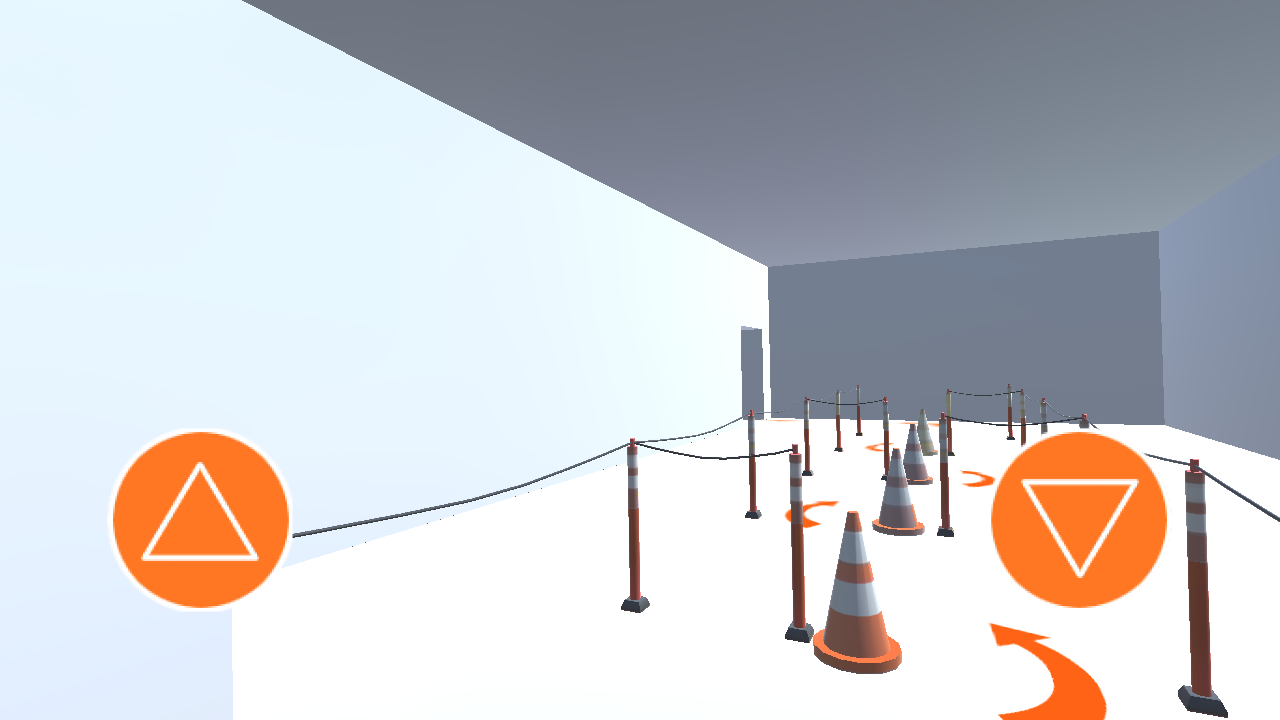
\includegraphics[width=.7\linewidth]{gyro1.png}
  \captionof{figure}{Initial sketch of gyroscope 1}
  \label{fig:test1}
\end{minipage}%
\begin{minipage}{.5\textwidth}
  \centering
  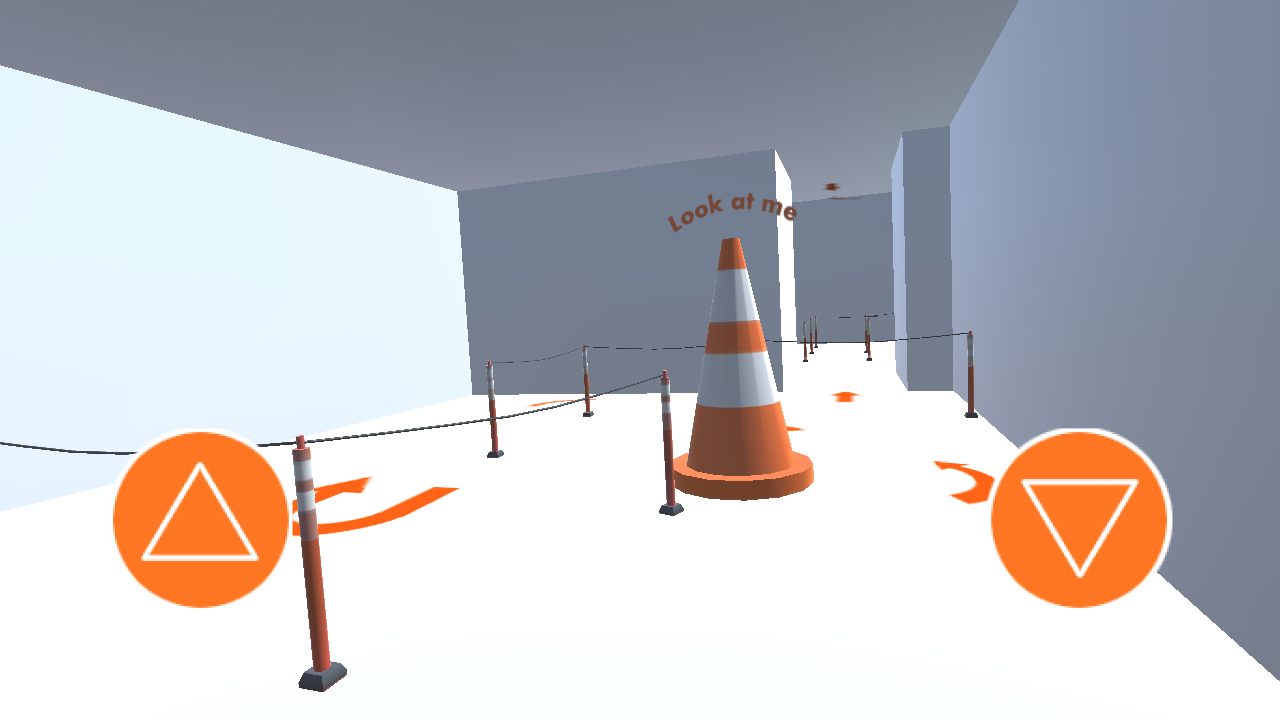
\includegraphics[width=.7\linewidth]{gyro2.png}
  \captionof{figure}{Initial sketch of gyroscope 2}
  \label{fig:test2}
\end{minipage}
\end{figure}


\subsubsection{Joystick}
In this prototype the user has to navigate using two joysticks - one for movement and one for camera movement/rotation. This should be easy to learn for the users that have experienced using a joystick before, and the target group is expected to have some knowledge as of how a joystick is supposed to work, because of their popularity in arcade and electronic games, where joysticks are placed on game console’s remotes like Sony Playstation series or Microsoft Xbox. Additionally, even for users with no previous joystick controller experience, that should not be a problem, as the control scheme is supposed to borrow the same concept as moving a computer mouse on the screen in the direction that is same as the device movement itself - both use 2d directional movement.

\begin{figure}[H]
\centering
\begin{minipage}{.5\textwidth}
  \centering
  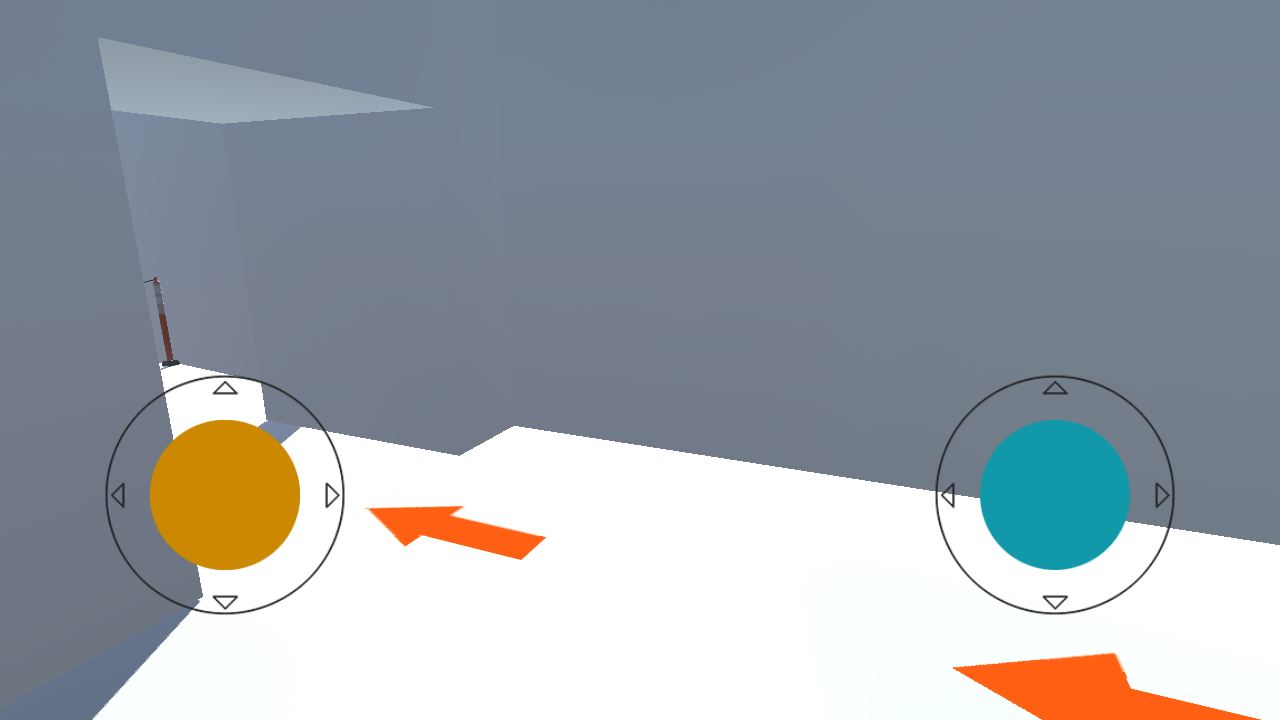
\includegraphics[width=.7\linewidth]{joystick1.png}
  \captionof{figure}{Initial sketch of joystick 1}
\end{minipage}%
\begin{minipage}{.5\textwidth}
  \centering
  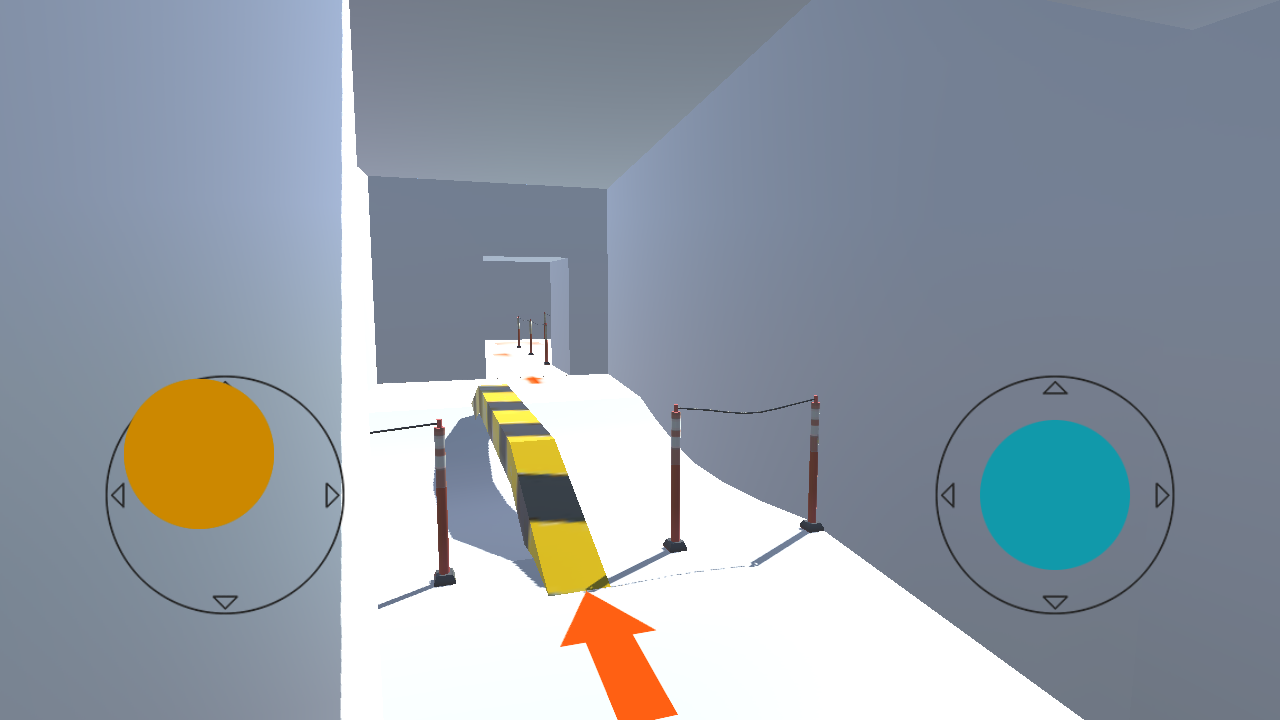
\includegraphics[width=.7\linewidth]{joystick2.png}
  \captionof{figure}{Initial sketch of joystick 2}
\end{minipage}
\end{figure}

\subsubsection{On-screen Buttons}
The way that should be the most familiar with the users through daily use - only buttons as the way to move both camera and the character. In this case camera would be moved only with arrow keys located on the screen and same for moving around - arrows indicating movement back and forth. This should be familiar with anyone that has used buttons for navigation of any sorts in virtual environment.

\begin{figure}[H]
\centering
\begin{minipage}{.5\textwidth}
  \centering
  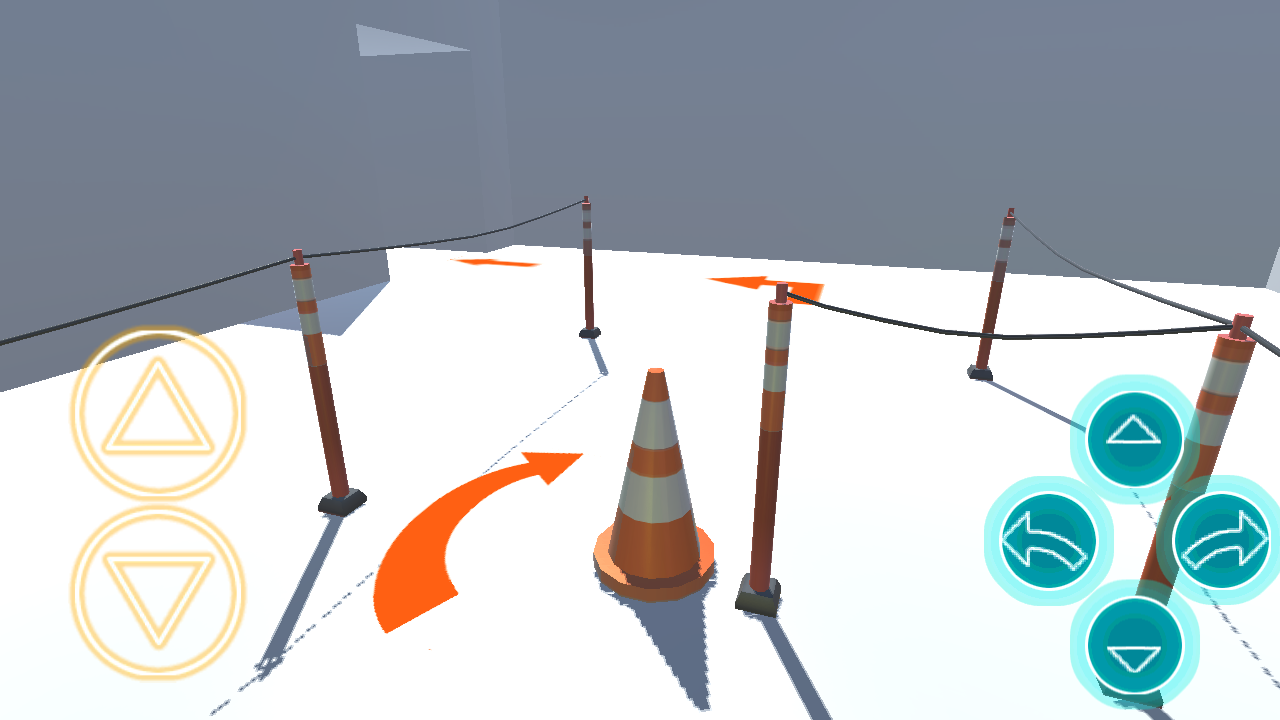
\includegraphics[width=.7\linewidth]{buttons1.png}
  \captionof{figure}{Initial sketch of buttons 1}
\end{minipage}%
\begin{minipage}{.5\textwidth}
  \centering
  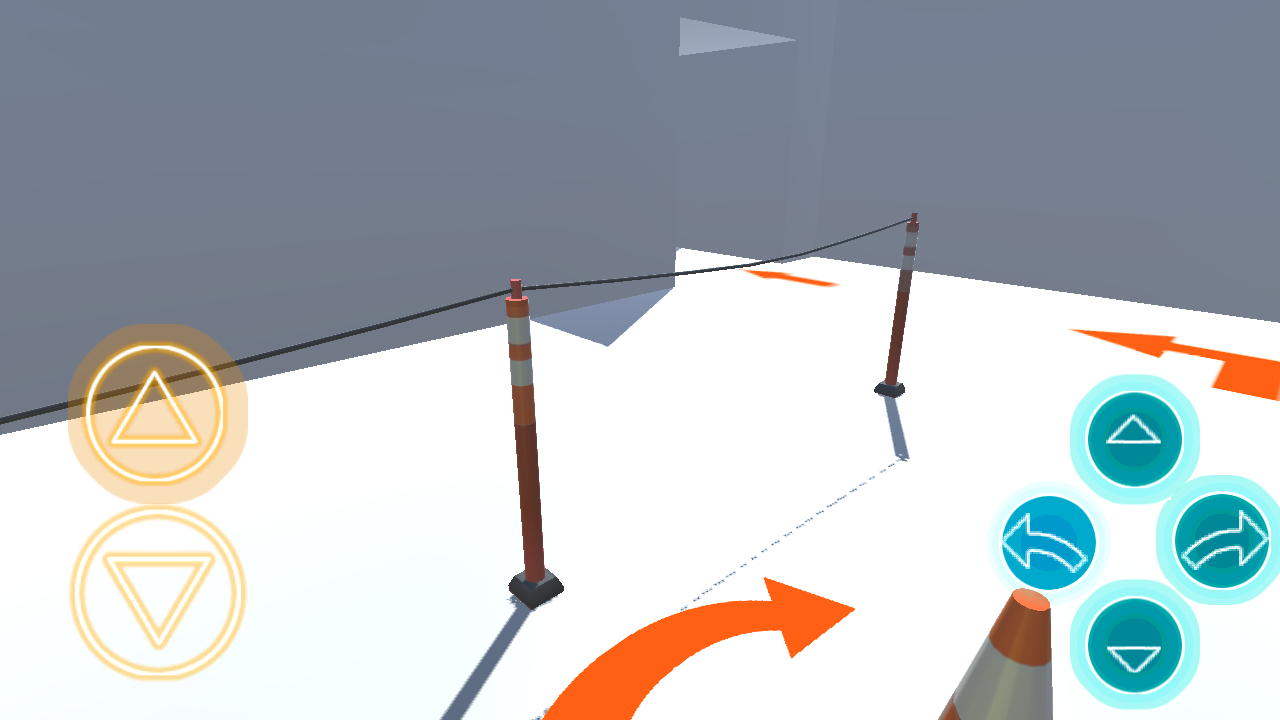
\includegraphics[width=.7\linewidth]{buttons2.png}
  \captionof{figure}{Initial sketch of buttons 2}
\end{minipage}
\end{figure}


By implementing familiarity concept to navigation, the problem of minimizing the knowledge gap is tangled so that the user is being trained in a way that seems natural.



\subsection{Isolation}
To further emphasize on the initial design requirements, the concept of isolation (\ref{GraphicalDesignIsolation} should be used when designing the controllers - this is done by making them stand out from the level content. This is supposed to help the user understand what parts of the application give feedback upon interaction.

\subsection{Immediacy and Simplicity}
To communicate information in a simpler, and faster to perceive manner, the designs should be represented by concepts that are already familiar to the user. This means, that to communicate information to the user, graphical elements should be represented as symbols that indicate either movement or rotation for buttons, and controls that represent an actual joystick, rather than
text. At the same time, this emphasizes the concept of affordance \ref{UsabilityAffordance}, as the buttons represent	mechanical buttons used in traditional types of controllers, as well as with the joystick controls. This will further shape the familiarity and intuitivity for the application (\ref{UsabilityAffordance}.

\begin{figure}[H]
\centering
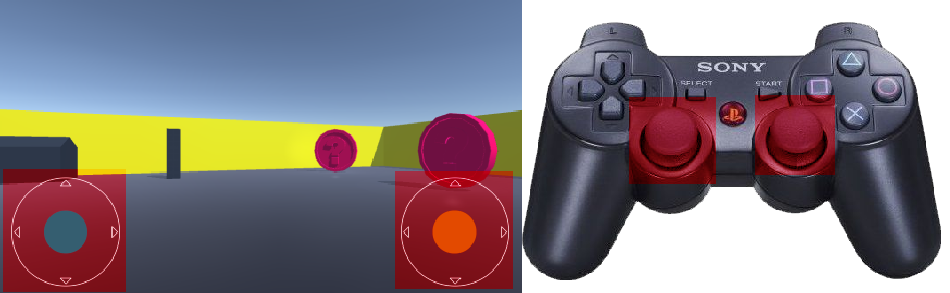
\includegraphics[scale=0.45]{JoystickComparison.png}
\caption{Comparison of initial design sketch of on-screen joystick and the Sony Playstation controller}
\end{figure}

\subsection{Graphical element sizes and placement}
To further emphasize on the user experience, the button size should be set accordingly - to	(ref
to UX ensure that the users would not have difficulties by unintentionally tapping the wrong section tetraple-gia stuff) of the controls, individual buttons have to be separated from each other and given the sizes for easy accessibility to reduce the “Fat Finger” problem. To enable a bigger view of the environment horizontally, the application will be built to primarily be viewed when holding the device in a landscape mode. Since the device is supposed to be held sideways and by both hands, all of the interaction should be done on the sides of the screen, for ease of control access.
To show the difference between movement and rotation controls, they should be given different looks - shape of directional arrows for buttons as well as color indication for both buttons and joystick controls.

\begin{figure}[H]
\centering
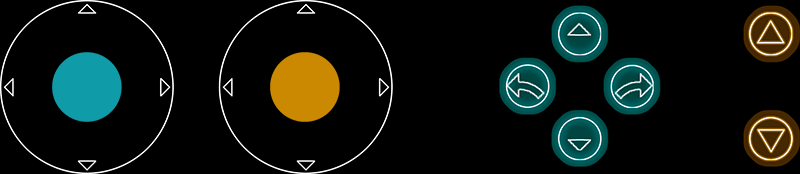
\includegraphics[scale=0.65]{ControllerColors.png}
\caption{Initial sketch. Color differences to distinguish controllers that hold different functions}
\end{figure}

\subsection{Design of 3D testing area}
To test different non-traditional control schemes 3D test area was designed. It consists of twisted path that test participants had to walk through as fast as possible \ref{TestLevels}.
\begin{figure}[H]
\centering
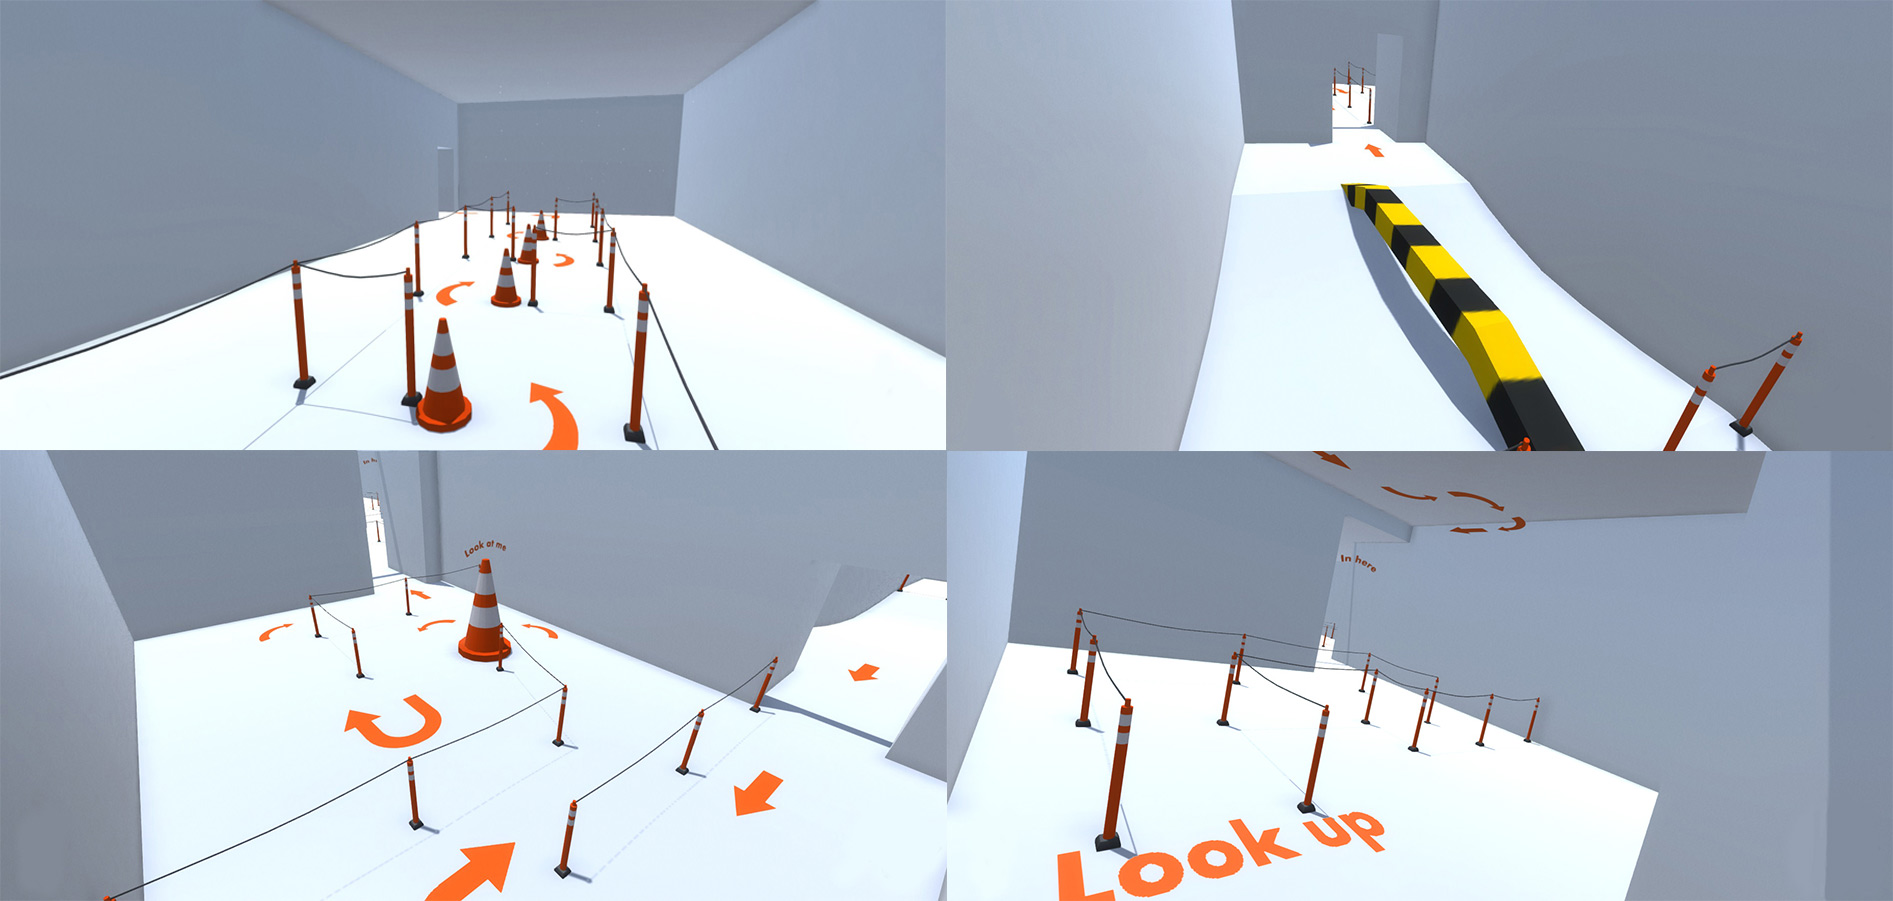
\includegraphics[scale=0.26]{3D_dev_6.jpg}
\caption{Pictures of the testing area}
\label{TestLevels}
\end{figure}
Focus of testing area was only on navigation for different schemes, so effort was placed on path and tasks and not on environment itself. All not important bits of the area were colored white and important as navigational arrows, cones and poles, explanatory text notes colored with sharp contrasting colors as red and orange. The “familiarity” consideration was done - navigational buttons and important bits on the level were kept in similar color, to help user recognize and focus on the purpose.
Analysing SOTA’s applications gave understanding what important aspects of navigation is. Firstly walking fluently around obstacles as furniture, doors, narrow paths. First two levels were developed for this to test. Second consideration was that users need to look around placed furniture which was not considered in most SOTA analyzed applications. Small area with huge cone and text “look at me” was placed and arrows in circular path around it. This represents how user would walk around furniture and inspect it by looking - focusing on one point while walking around \ref{TestLevel3}.
\begin{figure}[H]
\centering
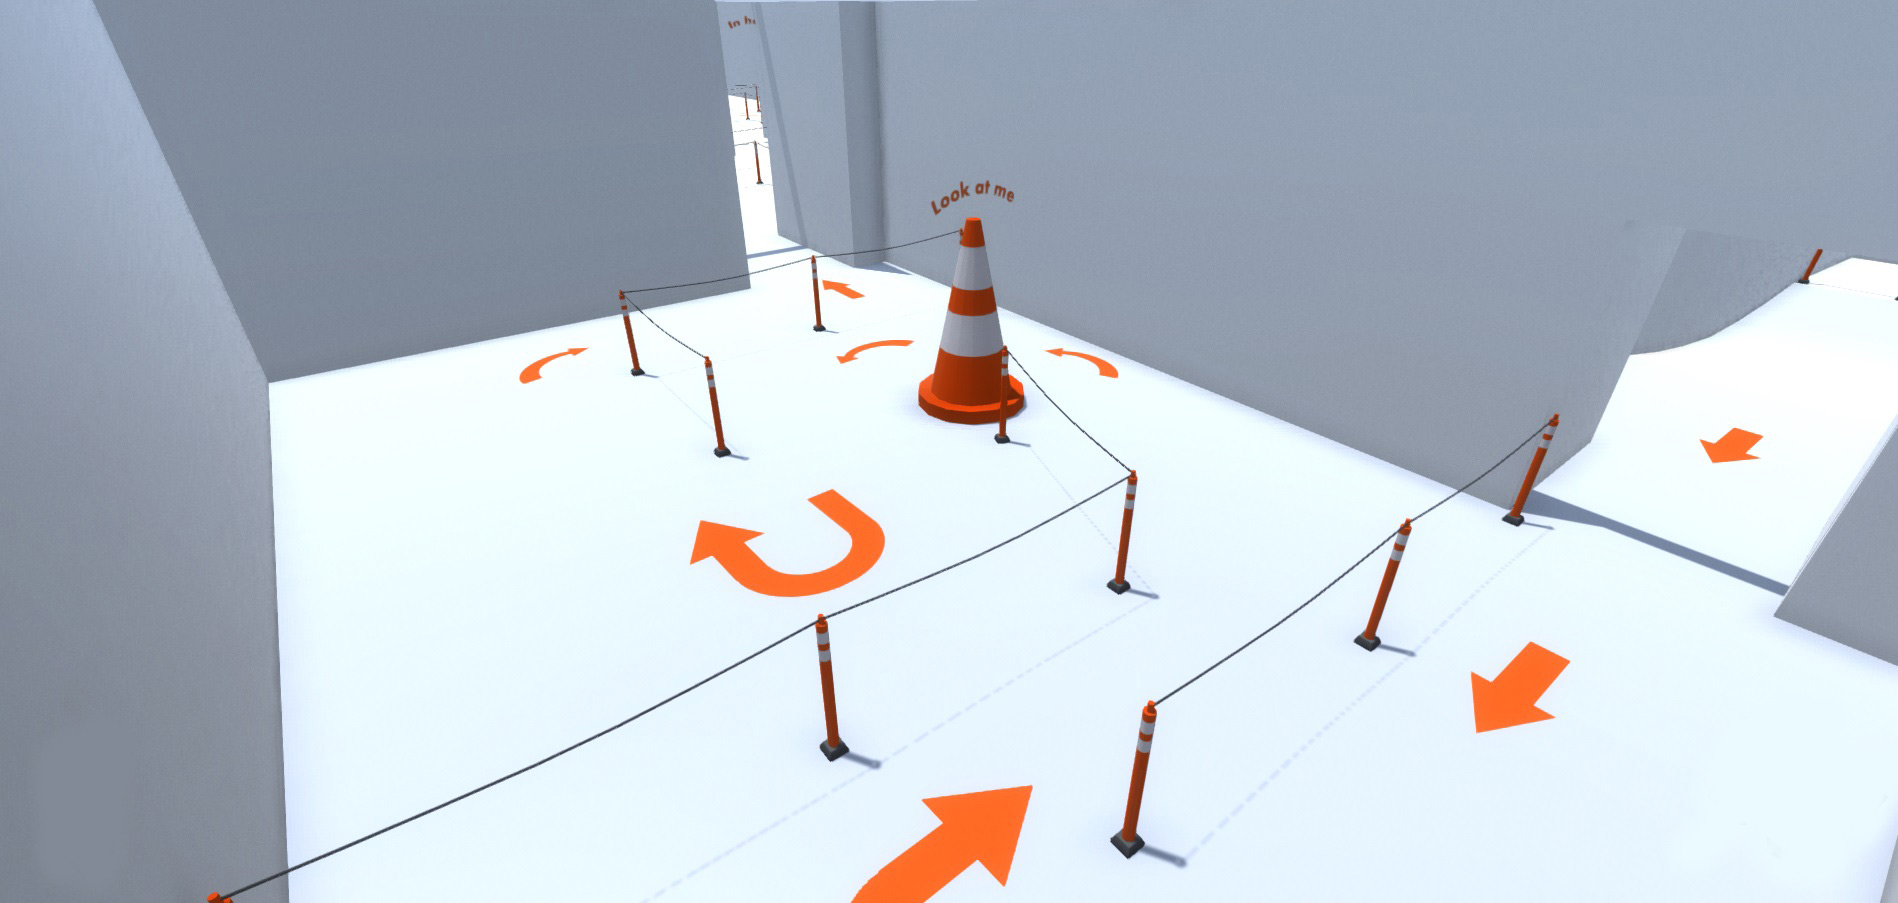
\includegraphics[scale=0.25]{3D_dev_3.jpg}
\caption{Third level of testing area. This level is to test how well user walks around an object.}
\label{TestLevel3}
\end{figure}
Next two levels were developed to test how efficient it is to look up and down while walking in given direction. It helps to test how well user can walk and look down or up at the same time \ref{TestLevel4}.
\begin{figure}[H]
\centering
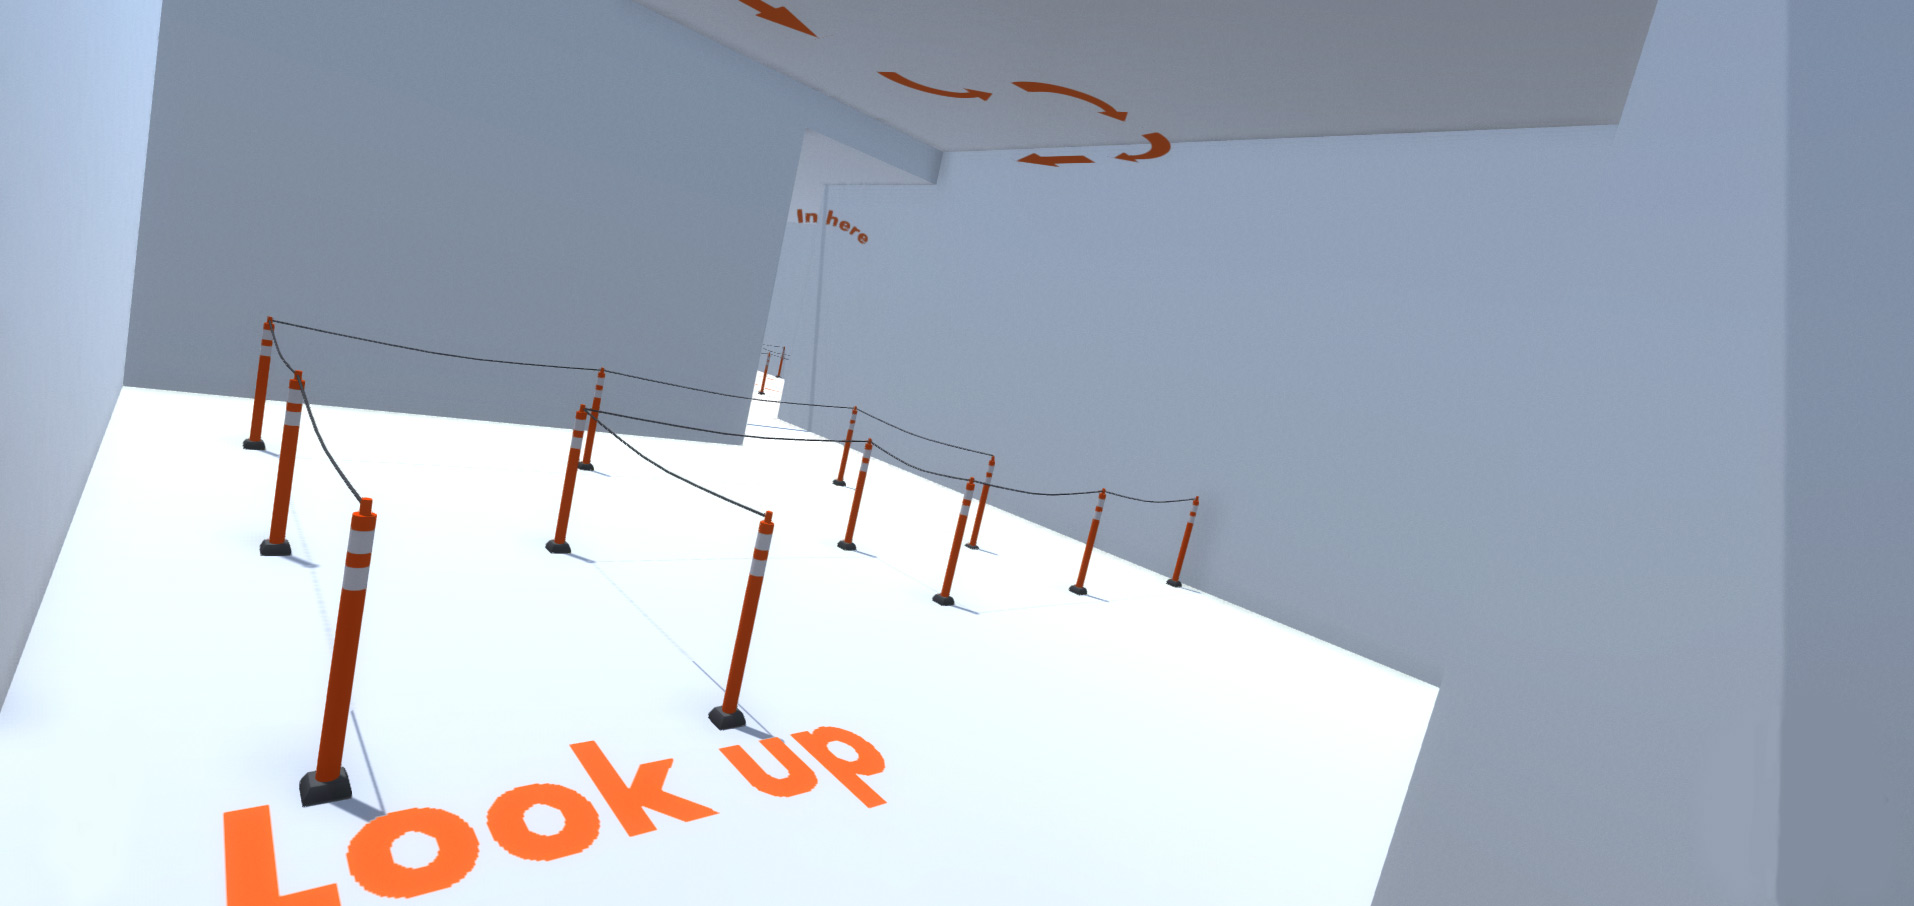
\includegraphics[scale=0.25]{3D_dev_4.jpg}
\caption{Test chamber to test how well user can walk and look up}
\label{TestLevel4}
\end{figure}
The last test area was created to see how user goes straight but looks to one side as the user would walk-by, but focus at some furniture aside \ref{TestLevel5}.
\begin{figure}[H]
\centering
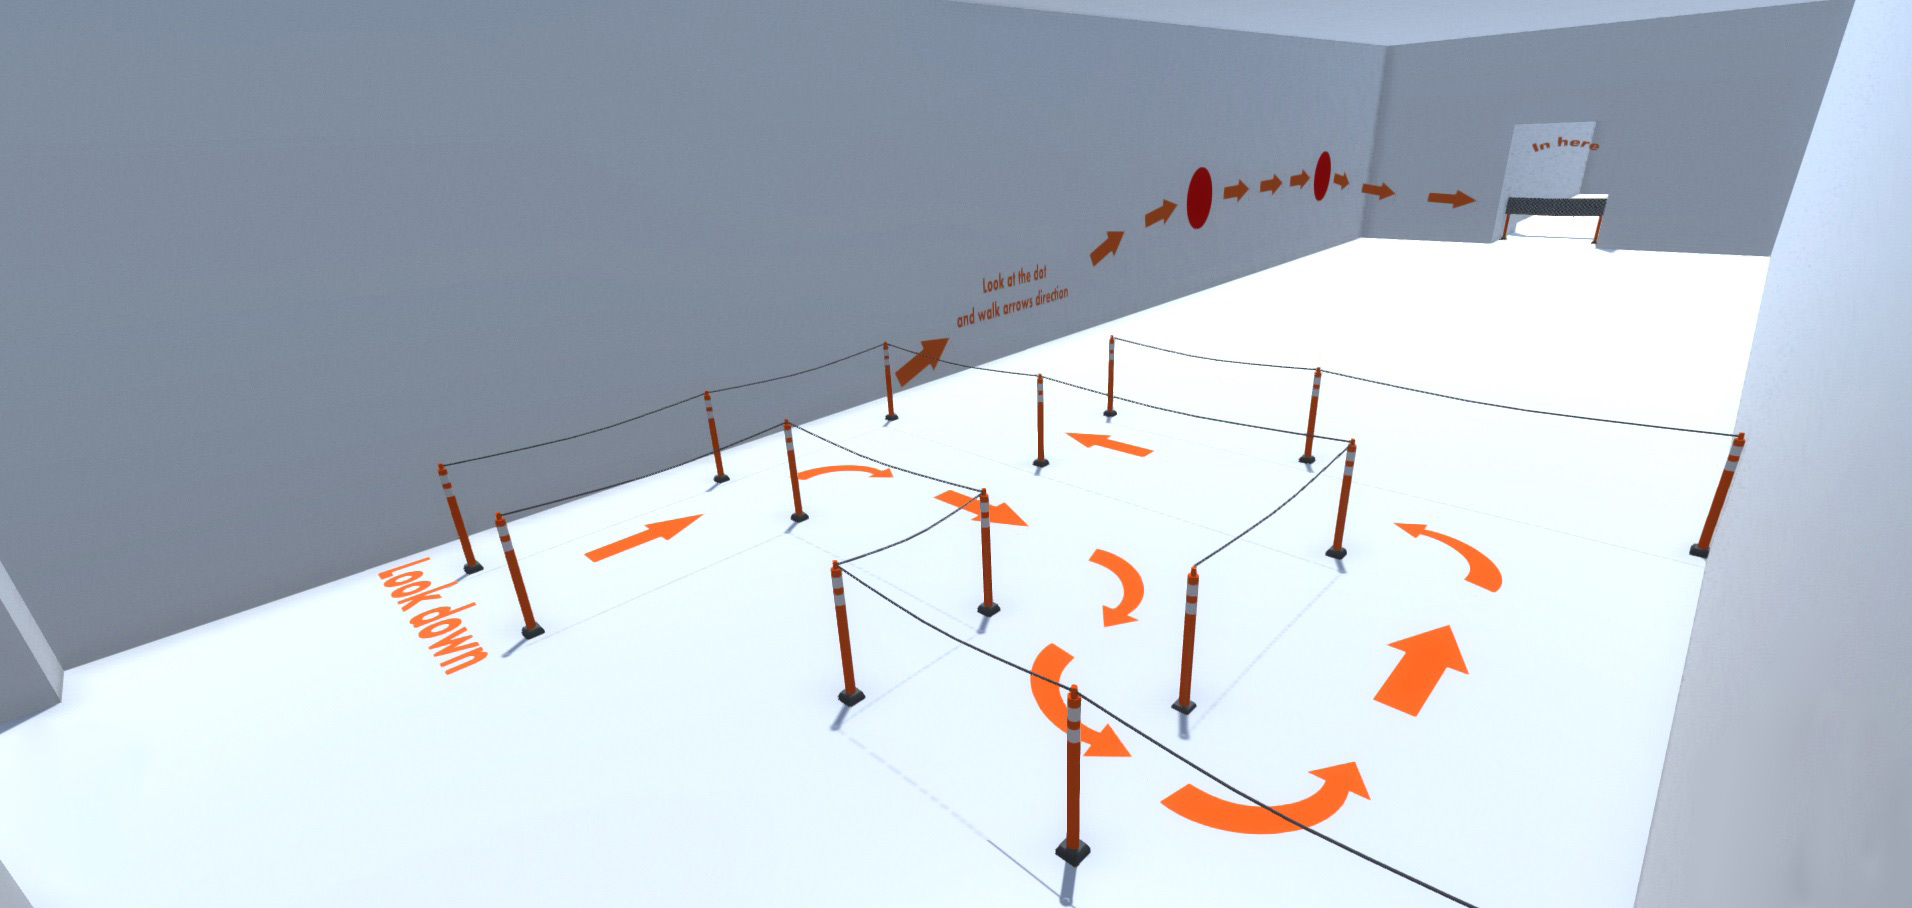
\includegraphics[scale=0.25]{3D_dev_5.jpg}
\caption{Last level of testing area. This level is to test how well user can walk while looking down and sideways}
\label{TestLevel5}
\end{figure}